\documentclass{article}
\usepackage{tabularx}
\usepackage[english]{babel}
\usepackage{blindtext}
\usepackage{listings}

\usepackage{graphicx} % Required for inserting images
\usepackage{array}
\renewcommand{\arraystretch}{2.5}
\title{PKS 2024 Project}
\author{Amal Akhmadinurov}
\date{October 2024}

\begin{document}

\maketitle
\tableofcontents
\newpage
\section{Introduction}
The project was written in the programming language C\#. Only standard .NET libraries were used.


\section{Protocol header}


\begin{tabular}{|p{2cm}|p{1cm}|p{1cm}|p{2cm}|p{4cm}|p{2cm}|}
\hline
Sequence Number (2b) & 
ID (2b) & 
Flags  (1b)& 
Filename Offset (2b) &
Data  &
Checksum (2b)

\\
\hline




\end{tabular}
\newline
\newline

\textbf{Sequence Number} is a 2 byte integer to store the number of the fragment. Used for Selective repeat ARQ method.
\newline

\textbf{ID}  is a 2 byte integer to distinct fragments of different messages. Assigned to a random number. Main purpose of this field is to make it possible to handle fragments from several message at the same time.
\newline

\textbf{Flags}  is a 1 byte containing the following flags (from the most significant bit to the leats significant bit):
\begin{itemize}
  \item Ack  
  \item Syn
  \item Last
  \item Keep-Alive
  \item File  
  \item Finish

 
\end{itemize}
\textbf{Ack} and \textbf{Syn} are used for setting up the initial connection and for requesting missing fragments.
\newline
\textbf{Last} flags indicates the last fragment of the message.
\newline
\textbf{Ping} and \textbf{Pong} are purposed to indicate signal message to keep the connection alive. The sender send message with Ping=1, while the receiver has to respond with message where Pong = 1.
\textbf{File} indicates file message.
\newline
\textbf{Finish} is used to terminate connection.
\newline
\textbf{Filename Offset}  is a 2 byte integer to indicate the amount of bytes in data part to be considered as filename. Ignored if File flag is 0.
\newline

\textbf{Data} contains data.

\textbf{Checksum} is a 2 byte fields containing CRC16 value to check the integrity of the message.

\section{Establishing and terminating connection}

\subsection{Establishing connection}
\begin{figure}[h]
    \centering
    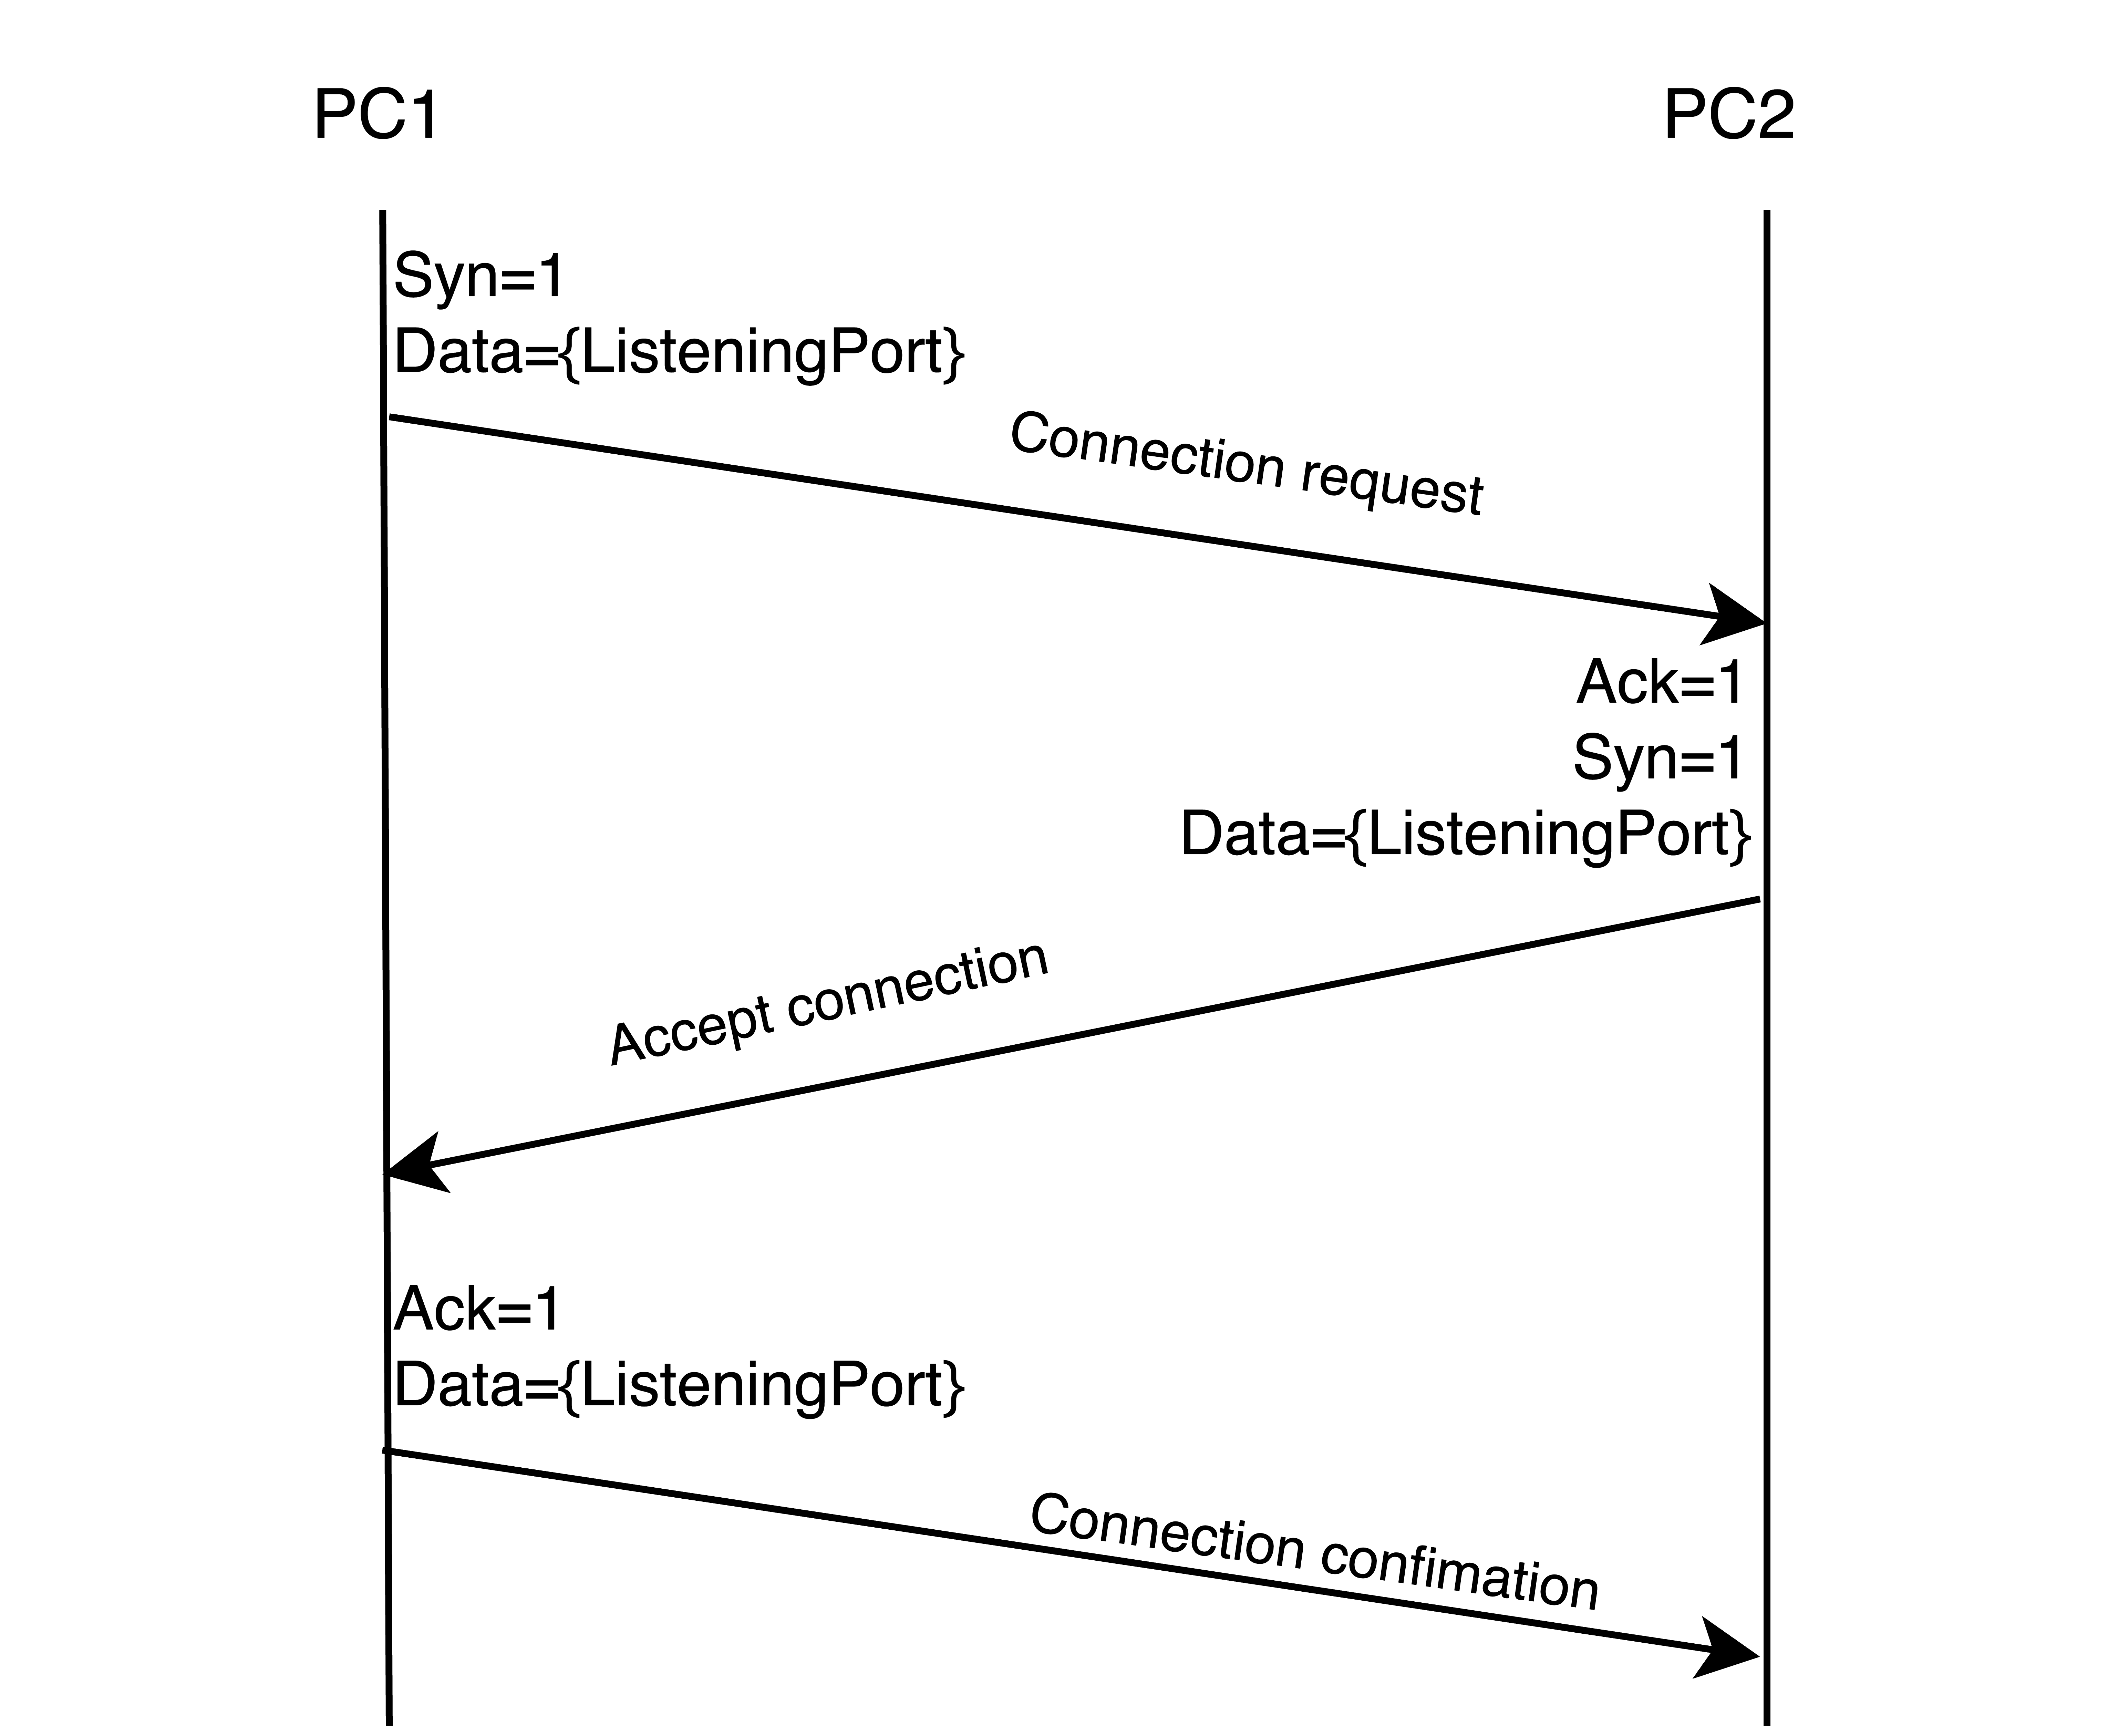
\includegraphics[width=\textwidth]{images/connection.png}
    \caption{Scheme of establishing connection}
    \label{fig:mesh1}
\end{figure}
Firstly, connection request is made (from PC1) to PC2. It contains flag Syn=1 and the listening port in Data.
\newline
PC2 responds back message indicating that  connection was accepted. This response contains flags Syn=1, Ack=1 and its own listening port as Data. PC2 now is waiting for the acknowledgement.
\newline
PC1 has to send acknowledgement , which is message with flag Ack=1.
\newline
After these steps connection is considered to be established.

\subsection{Terminating connection}

Terminating connection is done by sending request with flag Finish=1. After this connection is considered to be terminated.


\section{Keep-Alive}

\begin{figure}[h]
    \centering
    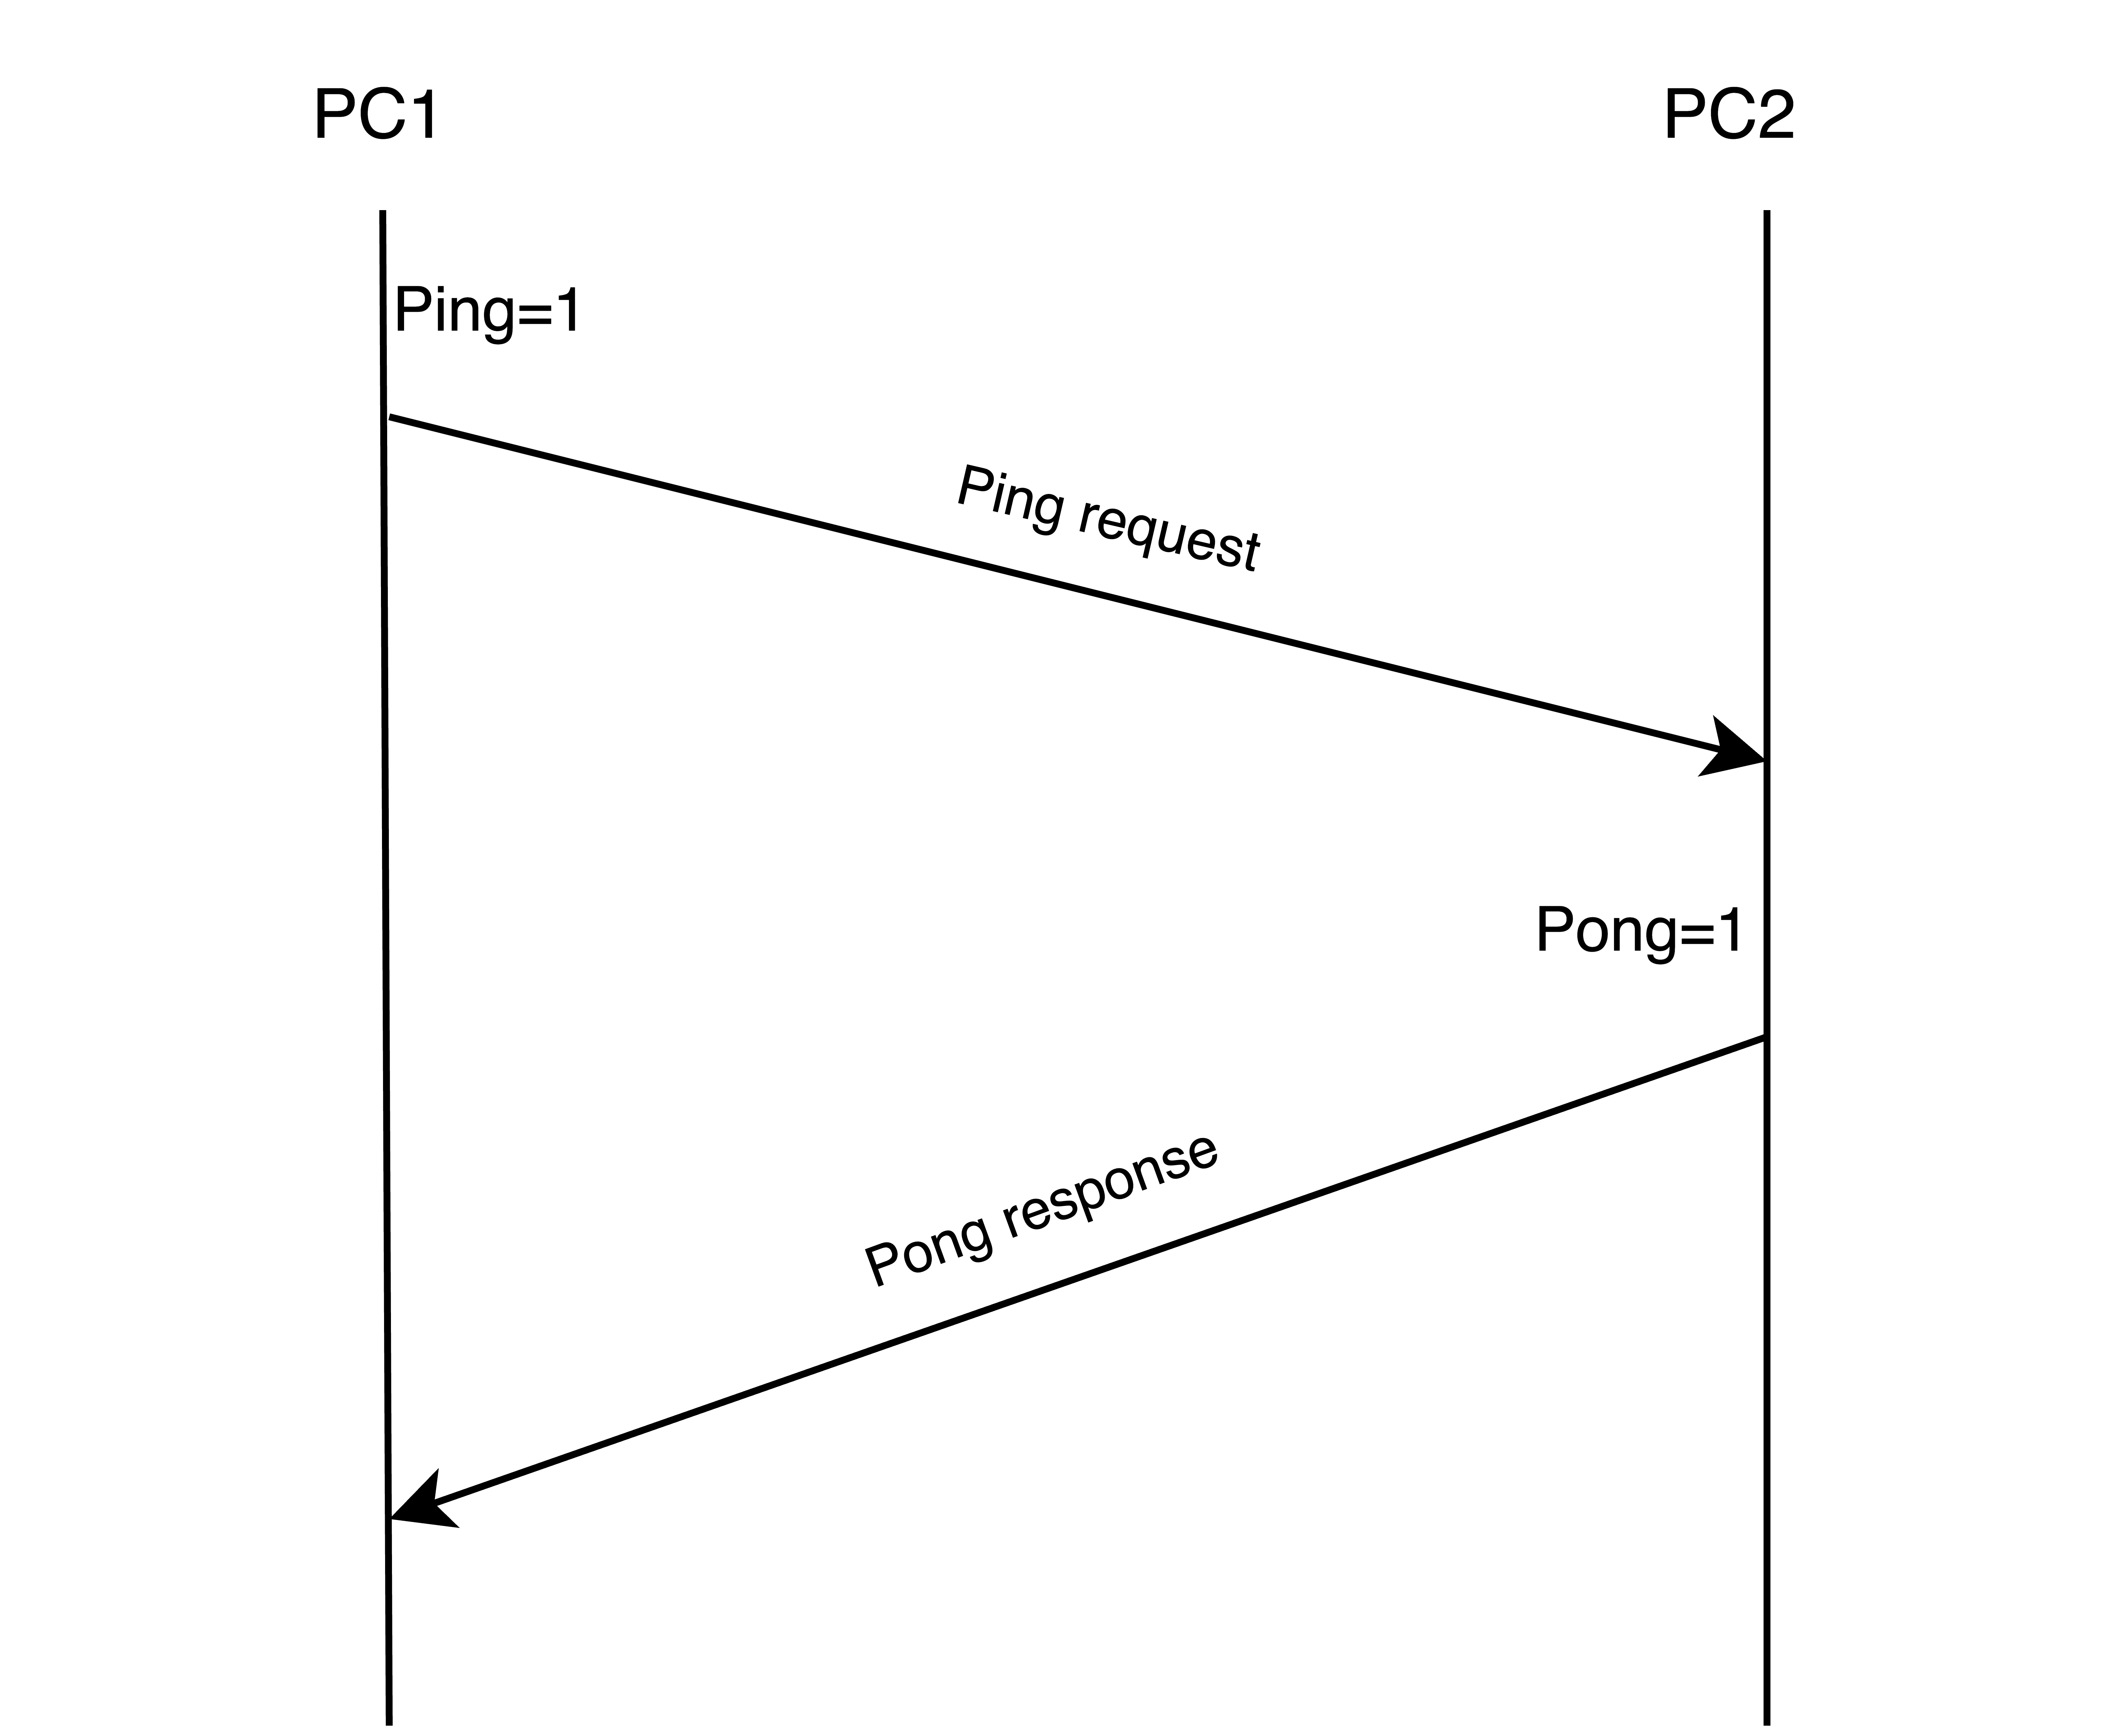
\includegraphics[width=\textwidth]{images/pingpong.png}
    \caption{Scheme of Ping-Pong request}
    \label{fig:mesh1}
\end{figure}
To keep the connection alive special message are used. Every 5 seconds each peer sends "Ping" request, that is a message with flag Ping=1 . The other side has to respond with flag Pong=1. After 3 consecutive unresponded "Ping" requests connection is considered to be lost and terminated.



\section{Data integrity}


\subsection{CRC16}

To control data integrity CRC16 algorithm is used. 
Own implementation of CRC16 is used.
During the computation algorithm will go  through every byte of data to be included in the message. Initially CRC is null. It will shift current CRC value by 8 to the right and perform XOR operation between current byte and CRC. Computed value is used as index for the lookup table. Value from the table is XORed with the CRC value shifted to the left by 8. This CRC value then is used for the computation for the next byte. CRC value that is computed for the last byte is the final value to be included in the Checksum part of the message. \newline
Lookup table is only an optimization for the whole algorithm. Assuming that byte can have only 256 values.
Table is filled with byte values after applying CRC key. Every byte is assigned to 2 byte int and shifted by 8, because CRC value is two byte value. After this the algorithm move though every bit of the byte: if the leading bit in the byte is null then it shifted by 1 to the left, if not it is shifted by 1 to the left and XORed with the value of the key. This step repeat 8 times for every byte value and the computed value put to the table, where index is the initial byte value and the value is the computed value.


\subsection{Selective repeat ARQ}
Selective repeat was chosen as ARQ method. 

\begin{figure}[!h]
    \centering
    \includegraphics[width=0.75\textwidth]{images/selectiverepeat.png}
    \caption{Scheme of Selective repeat ARQ for window size 4}
    \label{fig:mesh1}
\end{figure}

In the beginning, the sender sends several fragments (in this case 4, as window size is 4) without waiting for their acknowledgements, but starts timer every fragment.  Receiver acknowledges every frame it gets. After some period of time, sender understands that one of the fragments is missing acknowledgment and it resends the missing fragment. Every fragment can be resend several times. While the receiver is waiting, it still continue sending new fragments. For example if after initial 4 fragment were send and the first fragment is acknowledged,  the receiver moves its window by one fragment and can send the 5th fragment and so on. 

\pagebreak

\section{Program interface}
\subsection{Compile and run}

Open Project from src directory and open in Visual Studio Code, which will suggest steps to run it. In case it did't happen do the following:
\begin{enumerate}
\item https://dotnet.microsoft.com/ru-ru/download - download .NET SDK
\item Install C\# DevKit extension for VS Code
\item Install C\# extension for VS Code
\item Try run the projects
\end{enumerate}

\subsection{Usage}
Connection to the peer
\begin{lstlisting}
connect 127.0.0.1 -p 5050
\end{lstlisting}
Disconnection from the peer
\begin{lstlisting}
disconnect
\end{lstlisting}
Send simple text message
\begin{lstlisting}
send
\end{lstlisting}
Then input text to be sent

\end{document}
